\chapter{Framework for Comparing Time Series Classification Algorithms in Early Classification Context and Experimental Design}
\label{ChapterFrameworkExperiment}
This chapter describes our proposed framework which compares TSCAs in a context that is inspired by the problem of eTSC and the design of our experiment.
We begin by defining what we mean by early classification context and how does our framework simulate it.
Then we discuss the structure of the framework, the software tools that were used to build it and how to evaluate it.
In the second section of the chapter we represent our experimental setup.

%%%%
%%%%There are three research questions that are discussed:
%%%%\begin{itemize}
  %%%%\item How to adapt existing TSC workflows for the early TSC context ?
  %%%%\item How to evaluate classifiers in the early TSC context ?
  %%%%\item How to evaluate the proposed solution ?
%%%%\end{itemize}
%

\section{Framework for Comparing Time Series Classification Algorithms in Early Classification Context}
\label{SectionNewFramework}
%% Intro
As motivated earlier, eTSC is a field which is concerned with classification of time series data with earliness and accuracy
as the main objectives. Dedicated eTSCAs focus on building models that can learn class labels of the data as early as possible
while maintaining accuracy \cite{mori2017early}.
Our framework, on the other hand, investigates the adaptation of the context in which conventional TSCA operate to learn a specific
classification problem and the effect it has on the classifiers' performance. 

\subsection{Early Classification Context}
\label{SubsectionEarlyClassificationContext}
We define our early classification context as the problem in which a TSCA is trained on labeled but incomplete time series data, then
used to classify data instances of full length.

% This paragraph has been moved to the introduction
%The motivation behind experimenting with such a context is driven by the medical field, where sometimes patients have to go through strenuous tests to be diagnosed.
%This is specially the case in audiological examinations; as patients are exposed to signals which pushes the limits of their hearing discomfort to be able to examine their problems.
%A classifier which can attain comparable reasults while only learning on a fraction of the whole time series data would shorten this process and thus relief patients from their discomfort.

To answer our first research question \textbf{\textit{How can we adapt existing ts classification workflow for the early TS scenario ?}}

We propose a framework that simulates an early classification context by shortening the length of the data before learning classifiers on it,
then measuring the performance of the classifiers in comparison to their performance on full length data.
The framework divides whole timeseries data instances into smaller equal in length subseries using a chopping algorithm, then starts multiple learning processes.
The first learning process uses the first subsequence.
Then in each following learning process, the training data added the next subseuqnce in addition to the previous ones.
These processess simulate an incremental learning scenario, where the classifier is not exposed to all the data points collected from the beginning to the end at once, but in a sequential order.
In each learning process it gets to know more information about the data instances than the previous process.
To assess the performance of classifiers that were exposed to less data points, we use the performance of classifiers that were exposed to full length training data as a baseline.
In the next subsection \ref{SubsectionFrameworkStructureToolkits} we discuss the conceptual structure of the framework.


\subsection{Structure and Toolkits}
\label{SubsectionFrameworkStructureToolkits}
% Libraires we use
We implemented our framework in python language.
For the implementation of the non-deep learning algorithms we used the open source libraires $sktime V. 0.5.3$ \cite{loning2019sktime} and $pyts V. 0.11.0$ \cite{JMLR:v21:19-763},
while for the implementation of the deep learning algorithm InceptionTime we used the library $sktime\-dl V .0.2.0$ which provides an interface for the implementation provided
in the study \cite{fawaz2020inceptiontime}. Finally, we used the library $Tslearn V. 0.5.0.5$ \cite{JMLR:v21:20-091} as a mediator between the different model implementations; due to it's
capacity to process raw data into the needed input format by any of the libraries, as well as converting data format between the different libraires.

Our framework consists of two components; the comparison testbed and the recommender.
The testbed is the engine responsible for carrying out the comparisons.
It contains the

The testbed is the engine responsible for comparing the implemented algorithms on the data sets provided.
The testbed mainly collects user input about the experiment configuration, preprocesses the data in preparation for the learning process
and finally calculates performance metrics using testing data.
By the end of each performance assessment step, the testbed produces an analysis file and a logs file.
The logs file provides information about the setup of the experiment, the execution status, the duration and reasons of failure.
While the analysis file provides information about the cross validation scorese, the final hyperparameter values used, processing time of training and testing steps and the performance measures.

The second step of the framework is learning a recommender which will be able to predict the best performing algorithm(s) for an unseen data set.
Given the different analysis reports generated from the testbed, these reports are then consolidated and fed to the recommender to learn on.
First, the logging files are processed and filtered to get the data of the successfully executed processes.
Then the analysis files for these proccesses are consolidated into a unified structure and the included information is enriched by metadata about the data sets.
In the end, the data is preprocessed again to be fed to a regression classifier which learns from the results of already carried out experiments.
When given a new data set, the regression classifier tries to predict the performance of each implemeted classifier on the data set.
These scores are then used to rank the classifiers and the final recommendation is presented.

Our testbed component can be divided into several consecutive steps:
\begin{enumerate}
    \item User input
    \item Experiment preparation
    \item Experiment execution
    \item Analysis reports and logging
\end{enumerate}

In the next subsections, we will discuss the details and implementation of each step involved in the construction of our 2 steps framework.

\subsubsection{User Input}
\label{SubsectionUserInput}
% User Input
In the user input step, the user provides the necessary information required by the framework to start it's experiments.
These information provide the guidelines of the process which will be carried out and decide what steps should be done in the
experiment preparation step.
Table \ref{TableUserInput} shows a summary of each of the needed information, represented as a parameter for the framework.

\begin{table}[hbt!]
  \setlength\extrarowheight{2pt} % for a bit of visual "breathing space"
  \begin{tabularx}{\textwidth}{|X|X|X|}
  \hline
  \textbf{Parameter} & \textbf{Data Type} & \textbf{Description} \\ \hline
    Dataset         & String List        & The name of the data set(s)                        \\ \hline
    Splits          & Integer            & The number of splits to apply on the data set      \\ \hline
    Hyperparam      & Boolean            & Learn hyperparameters for the model or skip        \\ \hline
    NumIterations   & Integer            & Number of hyperparameters combinations to sample   \\ \hline
    ChunksToKeep    & Integer List       & The indexes of the chunks to use                   \\ \hline
    FromBeg         & Boolean            & Reveal data chunks from beginning or end           \\ \hline
    ScoringFunction & String             & The strategy for evaluating the model on test data \\ \hline
  \end{tabularx}
  \caption{Input parameters required for using the framework}
  \label{TableUserInput}
\end{table}

We implemented the user input interface using $docopt$ \footnote{https://github.com/docopt/}. A library which offers command-line interfaces through
the use of simple arguments and elements. It also allows setting default values for parameters which can be overriden if a value is passed.
In order to start running the framework, one provides the necessary parameter values through a simple terminal command.
Listing \ref{ListingUserInput} shows a sample command for running our master python file $run.py$ on the Computers data set using hyperparameters optimization,
while applying a split into 10 chunks.

\lstset{basicstyle=\ttfamily\small}
\begin{lstlisting}[language=Comsol,caption={Sample command for providing user input to the framework},captionpos=b,label={ListingUserInput}]
  python run.py --etsc --dataset=Computers --cv --split=10
\end{lstlisting}

\subsubsection{Experiment Preparation}
\label{SubsectionExperimentPreparation}
% Experiment Preparation
In the experiment preparation step, the framework starts preparing the different components of the experiment to be run.
These components include data set management, models initialization, preparation of the early classification context
and configuration of the training and testing processes.

% Datasets
Our framework's data sets handling module is configured to process data sets in either of two ways; automatic download from the UCR/UEA data archives,
or manually provided data sets that comply with some specifications.
Since the data loading module from $pyts$ \cite{JMLR:v21:19-763} offers integrated tools with the UCR/UEA data archives for fetching and downloading data,
we have configured our data module to extend $pyts$ by transparently checking both data archives when provided with a data set name.
The other option would be to provide a data set folder holding the name of the data set.
Inside the folder there should exist one training data set file with the name \enquote{FolderName\_TRAIN} and one testing data set file with the name \enquote{FolderName\_TEST}.
Which is the case for most of the data sets from both archives.
For multivariate data sets, our framework assumes that the training data set file, as well as the testing data set file, contains data of all dimensions.
For maximum compatibility, our framework extends the data processing utilities from $sktime$ \cite{loning2019sktime}
which can read data sets that comply with the guidelines provided by the UCR and the UEA archives.
We consider \enquote{arff} format as the primary expected data type.

%Multivariate (models initialization)
As mentioned earlier in section \ref{GreatBakeoffMultivariate}, there are two ways to work on multivariate time series data sets \cite{ruiz2020great}.
The first way is by using bespoke multivariate classifiers which can deal with the multiple dimensions available in the data.
While the other is by using ensembles of univariate classifiers, each fit to a separate dimension under the assumption of independence between the dimensions.
Our framework applies the second technique for handling multivariate data sets.

In the experiment preparation step, the framework checks the data and determines the number of dimensions in consists of.
If the data set is univariate then the model initalizes the default classifer implementations provided by the libraries.
In case the data set was found to be multivariate, we initialize a special classifier type which extends the usage of univariate classifiers for multivariate problems.
This special classifier is reffered to as $ColumnEnsembleClassifier$ in the $sktime$ library implementation and as the $MultivariateClassifier$ in $pyts$.

There are two assumptions that we make at this step in our framework.
First, we assume that to extend a specific univariate classifier to a problem, we should fit the same type of the classifer on all dimensions of the data.
This is goes back to our goal, that we want to compare classifiers from different groups and not to create an ensemble which makes use of different classifiers
applying different techniques, like HIVE-COTE does.
Second, we assume that we always have to fit one classifier per dimension, which have proved to be not a feasible solution for high dimensional data sets.
We will discuss this in more details in our results.

% Hyperparam + Scoring Function (configure training and testing)
In preparation for the following steps in the framework, the experiment preparation step plays a role in configuring the training and the testing processes.
For the training process, it is possible to either run using the default configuration of the classifiers from their libraries, or to learn it's hyperparameters through cross validation.
We use a randomized search over the hyperparameters space of classifiers.
The framework parameter $NumIterations$ represents the number of random samples to consider when optimizing the hyperparameters.
If the space of the hyperparameters is less than $NumIterations$, then the space is exhausted by applying a grid search. We have considered 5-folds cross validation for all experiments.

For the testing process, the framework allows the usage of any chosen performance metric which is supported by $sklearn$ library \cite{scikit-learn}.
The chosen performance metric is utilized for the evaluation during both; the cross validation process and for calculating performance on the test data set.
We consider \enquote{balanced accuracy} as our default performance metric; to account for problems where data sets have imbalanced classes distribution.

% Chopping Algorithm
Based on the assumption that all data instances are of the same length, we implement our early classification context using a time series chopping algorithm.
The algorithm is provided with some time series data set $T$ with instances of length $L$ and three user defined parameters; $s$ which decides the number of splits $L$ should be split to,
$FromBeg$ a flag which indicates whether the data chopping should occur from the beginning or the end of the time series $T$, and $ChunksToKeep$ which provides the user
with the option to use only specific chunks of interest and exclude the processing for all other chunks.
Algorithm \ref{AlgorithmChopping} demonstrates how the chopping algorithm works.

The result of the algorithm is then used to create new copies of $T$; $[T_{1}, T_{2}, \ldots, T_{s}]$, each copy $T_{i}$ containing all instances from $T$ but revealing a subsequence of $L$
which we call the chunk. A chunk is a sequence of $p$ data points starting from the beginning or the end of the instances in $T$ based on the value of the parameter $FromBeg$.
Each data set copy $T_{i+1}$ reveals one more chunk than the previous data set $T_{i}$ and the data set $T_{s}$ represents the set with instances of the full length $L$.
It should be noted that our algorithm tries to have an equal value for $p$ used for each chunk, but this is limited by the length of the time series and the provided number of splits.
The resulting data sets are then passed to the training process, where each algorithm applies it's own technique to learn on the data set.

\begin{algorithm}
    \caption{The Chopping Algorithm}\label{AlgorithmChopping}
    \begin{algorithmic}[1]
      \Function{$GetSplitIndexes$}{$T,s,ChunksToKeep$}
        \State $L \gets ExtractLength(T)$
        \State $ChunksSizes \gets GetChunkSizes(L,s)$
        \State $SplitIndexes \gets CumSum(ChunksSizes)$
        \If{$KeepChunks$ is not Null}
                \State $FilteredSplitIndexes \gets KeepChunks(SplitIndexes,ChunksToKeep)$
            \Else
                \State $FilteredSplitIndexes \gets SplitIndexes$
            \EndIf
        \State \textbf{return} $FilteredSplitIndexes$
      \EndFunction
    \end{algorithmic}
\end{algorithm}

To better understand how the chopping algorithm works, consider the next example.
Let's assume we have a data set $T$ with instances of length $L$ = 100, we set the value of $s$= 10 and $FromBeg$ = True.
The algorithm starts by calculating the value of $p$ for each of the required 10 chunks using the function \ref{FunctionChunkSizes}.

\begin{algorithm}
    \caption{Function to Get Chunks Sizes}\label{FunctionChunkSizes}
    \begin{algorithmic}[1]
      \Function{$GetChunkSizes$}{$L,s$}
      \State $ChunksSizes \gets$ [ ]
        \For{\texttt{$i \gets 0$ to $s-1$}}
            \If{$i < L\pmod{s}$}
                \State $p = (L \div{s}) + 1$
            \Else
                \State $p = L \div{s}$
            \EndIf
            \State $ChunksSizes.append(p)$
        \EndFor
        \State \textbf{return} $ChunksSizes$
      \EndFunction
    \end{algorithmic}
\end{algorithm}

The resulting list $ChunksSizes$ from the algorithm will contain the value 10 for each of the chunks ($ChunksSizes$ = [10, 10, 10, 10, 10, 10, 10, 10, 10, 10]);
this is because the length of the time series is divisible by the number of splits provided, so it results in perfect splits of the data and thus chunks of equal sizes.
If we assume the same scenario again but with a different $s$ value like 8, the algorithm will try to provide as equal values of $p$ as possible
giving back a $ChunksSizes$ of values [13, 13, 13, 13, 12, 12, 12, 12].

After calculating the chunk sizes, the chopping algorithm translates $ChunksSizes$ into a list of indexes called $SplitIndexes$.
Which is then used to create the different copies $T_{i}$ by selecting subsequences.
The values of $SplitIndexes$ are the indexes of the last time point that a specific chunk should read.
We calculate these values by carrying out a cumulative sum over the values of $ChunksSizes$.
For example, the list $ChunksSizes$ = [10, 10, 10, 10, 10, 10, 10, 10, 10, 10] is translated into the list $SplitIndexes$ = [10, 20, 30, 40, 50, 60, 70, 80, 90, 100].
This means that the corresponding data set $T_{1}$ will contain all it's data instances represented by the subsequences from the \nth{1} time point till the \nth{10} time points,
and the data set $T_{3}$ will contain subsequence from the \nth{1} time point till the \nth{30} time point.
When we apply the same translation to the list $ChunksSizes$ = [13, 13, 13, 13, 12, 12, 12, 12], it gets translated into $SplitIndexes$ = [13, 26, 39, 52, 64, 76, 88, 100].

Finally, the algorithm filters out the list $SplitIndexes$, if the user provided a list of specific chunks to keep using the variable $ChunksToKeep$.
The values passed through $ChunksToKeep$ corresponds to the indexes of the chunks the user is interested in, all the other chunks are excluded.
Note that this process is different from reducing the number of splits; as the number of splits affects the sizes of the chunks being created.
While $ChunksToKeep$ is used only to filter out the chunks after their sizes are already determined and translated into $SplitIndexes$.
The space of possible values for $ChunksToKeep$ is between [1, $s$]. The logic of the function is demonstrated in function \ref{FunctionChunksToKeep}

\begin{algorithm}
    \caption{Function to filter out Chunks}\label{FunctionChunksToKeep}
    \begin{algorithmic}[1]
      \Function{$KeepChunks$}{$SplitIndexes,ChunksToKeep$}
      \State $FilteredSplitIndexes \gets$ [ ]
        \For{\texttt{$i$ $\epsilon$ $ChunksToKeep$}}
                \State $FilteredSplitIndexes.append(SplitIndexes[i])$
        \EndFor
        \State \textbf{return} $FilteredSplitIndexes$
      \EndFunction
    \end{algorithmic}
\end{algorithm}

If we consider the list $ChunksToKeep$ = [1, 3, 5] for our example $SplitIndexes$ = [10, 20, 30, 40, 50, 60, 70, 80, 90, 100].
The resulting filtered list will be $FilteredSplitIndexes$ = [10, 30, 50], which will result in only 3 copies of $T$; $T_{1}$, $T_{3}$ and $T_{5}$,
each represented by it's respective subsequence length.

% Relation between s and the earliness
If we have a closer look at the parameter $s$, we can recognise that it contributes to the granularity of the earliness factor that we are calculating.
The value of $s$ decides the total number of chunks we will use, which subsequently decides also the ratio represented by each chunk to the total length of the time series $T$.
That means the greater the value of $s$, the smaller the chunk sizes and consequently the more granular results we can test for the algorithms.
If we consider our previous example, when we set the value of $s$ = 10 then the length of each subsequence would be close to 10\% of the total length.
If we decided to change the value of $s$ = 20, then each chunk will roughly represents 5\% of the total length and so on.
Increasing the number of splits to be used comes with the cost of time and resources, each extra split adds one extra run per algorithm per data set.

\subsubsection{Experiment Execution}
\label{SubsectionExperimentExecution}
% Training Models
The experiment execution step is where the actual processing happens.
After the preparation of the chunks for the data sets in the previous step, learning processes start and each of the implemented classifiers starts training on the prepared data sets.
Each of these training processes is then followed by a testing process, where performance scores are calculated using the function provided by the parameter $ScoringFunction$ on testing data sets.

As mentioned in section \ref{SectionTSCA}, we follow the grouping criteria by \cite{bagnall2017great} which arranges TSCAs into 5 main categories based on their techniques.
We have included classifiers representing each of the 5 groups, in addition to a \nth{6} group which represents the family of deep learning time series algorithms.
We tried, as far as the implemented libraries allowed, to represent each group with 2 classifiers; one that is a non-ensebmle and another which is an ensemble.
A total of 10 classifiers are included in the framework covering all 6 groups, these can be broken down into the following:
\begin{itemize}
  \item Distance based : 1NN using MSM distance and PForest
  \item Phase dependent algorithms : TSF
  \item Shapelets: LS and ST
  \item Dictionary based : WEASEL and BOSS
  \item Deep learning : InceptionTime
  \item Classical baselines: 1NN using euclidean distance and 1NN using DTW
\end{itemize}

Table \ref{TableClassifierParams} shows the configuration and hyperparameters for all the included classifiers.
We used the same hyperparameter space like that of the original published papers as closely as possible.
During training, the number of hyperparameter sampling is decided by the framework parameter $NumIterations$ and we fix the number of cross validation folds to 5.

\begin{table}[hbt!]
  \setlength\extrarowheight{2pt} % for a bit of visual "breathing space"
  \begin{tabularx}{\textwidth}{|X|X|}
  \hline
  \textbf{Classifier} & \textbf{Parameters} \\ \hline
  MSM                 & c = \{0.01, 0.1, 1, 10, 100\}                                                        \\ \hline
  PForest             & k = 100 \newline r = 5                                                               \\ \hline
  TSF                 & r = 500 \newline splitting = \{entropy, gini\} \newline maxfeatures = \{sqrt, log2\} \\ \hline
  LS                  & $\lambda_{w}$ = \{0.01, 0.1, 1\} \newline
                        $L_{min}$ = \{0.025, 0.075, 0.125, 0.175, 0.2\} \newline R = \{1, 2, 3\} \newline
                        K = \{0.05, 0.15, 0.3\} \newline $\eta$ = 0.01 \newline
                        maxIter = \{2000, 5000, 10000\}                                                      \\ \hline
  ST                  & t = 60 mins \newline n=\{500,100\}                                                   \\ \hline
  CBOSS               & t = 60 mins \newline k=\{50, 100, 250, 500\} \newline s=250 \newline p=[0.5 - 1]     \\ \hline
  WEASEL              & ANOVA = \{True, False\} \newline bigrams =\{True, False\}
                        \newline binning = \{equi-depth, equi-width, information-gain\}                      \\ \hline
  Inception           & epochs = 1500 \newline batch size = 64 \newline $\eta$ = 0.001 \newline
                        kernel sizes = \{10, 20, 40\}                                                        \\ \hline
  DTW                 & full warping window                                                                  \\ \hline
  \end{tabularx}
  \caption{Parameters and configuration for TSCAs}
  \label{TableClassifierParams}
\end{table}

After the training processes are finished, the classifiers are then shown the testing data sets to evaluate their performance.
If the experiment is configured to do hyperparameter optimization,
then the classifier version that attained the highest validation score, from the 5 cross validation folds, is used for calculating the performance score on the testing data set.


\subsubsection{Analysis Reports and Logging}
\label{SubsectionAnalysisReport}
% Analysis Report
The last step of our framework is the analysis report preparation.
After the successful running of the experiments and calculating performance scores using the provided scoring function, we create a single report for each run experiment.
We produce one report per classifier per data set.
We refer here by data set to each data set that was finally produced by the chopping algorithm.
These reports collect the essential data and statistics that form the basis of our results.
Table \ref{TableAnalysisReport} shows the structure of the output for the analysis report.

\begin{table}
  \setlength\extrarowheight{2pt} % for a bit of visual "breathing space"
  \begin{tabularx}{\textwidth}{|X|X|}
  \hline
  \textbf{Item} & \textbf{Description} \\ \hline
    Classifier                 & The classifier name                                             \\ \hline
    Train time                 & The total training time (CPU Time)                              \\ \hline
    Test time                  & The total testing time (CPU Time)                               \\ \hline
    Test score                 & Performance score on testing data set                           \\ \hline
    Params                     & List of hyperparameters used and their values                   \\ \hline
    Revealed \%                & Percent of data points used for training from the total length  \\ \hline
    F-score                    & $F_{\beta}-measure$ between test score and revealed \%          \\ \hline
    Data set                   & The name of the data set                                        \\ \hline
  \end{tabularx}
  \caption{Analysis report created for each experiment}
  \label{TableAnalysisReport}
\end{table}

Most of these information are already available once the testing process is finished; because either they are metadata about the experiment or metrics calculated during training and testing.
Metadata about the process is already known before the running of the process; like the $Classifier$, $Data set$ and $Revealed \%$.
While the processes metrics are $Train time$ , $Test time$; which represent the total duration of the learning and testing processes, and the $Test score$ which represents performance of the classifier.


There is only one metric which is calculated during the analysis report phase after all the other metrics are calculated; the $F_{\beta}-measure$.
We previously defined the $F_{\beta}-measure$ in chapter \ref{EarlyTimeSeriesClassification}, it has been used, in the form of $F_{1}-Score$, by \cite{schafer2020teaser} as the objective function for evaluating their algorithm $TEASER$.
The $F_{\beta}-measure$ is a popular choice for calculating a score that combines 2 objectives at the same time, which are earliness and performance for eTSC problems.
Likewise, we use $F_{\beta}-measure$ as the means of evaluating classifiers in our experiments; due to it's capacity to incorporate both objectives in one score.
Which allows us to compare the trained classifiers in terms of a one score value without worrying about fixing the value of either the earliness or the performance,
as well as changing assigning different weights for the objectives if needed.


On the other hand, the $F_{\beta}-measure$ equation that was discussed in chapter \ref{EarlyTimeSeriesClassification} doesn't fit directly into our evaluation framework.
If we try to substitute the results for a classifier trained on the full length data into this equation, we would always get a value of 0.
The reason is that the equation is designed to do reverse scoring to the value or earliness, by re-coding its value so that the less seen data points, the higher the contribution of earliness in the equation.
This is simply achieved by using (1 - earliness) instead of using the value of earliness directly.
In case of calculating scores at full length, this would yield a value of 0 regardless of the performance of the classifier;
since the earliness value at full length is 1, then the equation (1 - earliness) would always give a 0 score causing the numerator to be 0.

Our modification to the $F_{\beta}-measure$ is a two fold procedure.
First, we reverse its scale, so that the lower the value the better. Then we reverse score the result again so that it returns to the original scale.
We represent our 2 steps modification in equations \ref{Equation:HMNew1} and \ref{Equation:HMNew2}.

\begin{align}
    & F_{\beta}-reversed =
        \begin{cases}
          1 & \text{if earliness = 1 $\land$ performance = 0} \\
          1 & \text{if earliness = 0 $\land$ performance = 0} \\
          (1 + \beta^2)\frac{\text{(1 - performance) earliness}}{\beta^2 \text{(1 - performance) + earliness}} & \text{otherwise} \\
        \end{cases} \label{Equation:HMNew1} \\
    & F_{\beta} \text{ = 1 - } F_{\beta}-reversed \label{Equation:HMNew2}
\end{align}

In the first step, we reverse the scale of the original $F_{\beta}-measure$ equation by changing its equation.
Instead of reverse scoring earliness and using the actual performance score value, we use the actual earliness value and reverse the performance metric score.
We name this measure the $F_{\beta}-reversed$, to clarify that it represents a reversed value of the $F_{\beta}$ used in other papers.
Using $F_{\beta}-reversed$, if we consider the case of classifiers learning at full length, 
it would solve the problem of attaining a score of 0 and replace it with a real value.

There are 2 special cases to be handled during this step.
First, if the classifier doesn't predict anything correct but at the earliest point in time.
Second, if the classifier doesn't predict anything correct while seeing the full length.
These two cases are then assigned the lowest value, which is 1.
In the second step, we reverse score the value from the first step again; to math the expected input for generating critical difference diagrams.
We feed these equation with the values of the features $Revealed \%$ and $Test score$, for the attibutes earliness and performance respectively.


\section{Experiments}
\label{SectionExperiment}
% Experiments
Our experiments were conducted on univariate data sets from the UCR archive as well as multivariate data sets from the UEA archive.
The data sets were chosen based on the criteria discussed in the subsection \ref{used data sets}.
Each of the data archives offers a train and test split of the data which we have used unchanged for all the classifiers.
All our experiments were run on a LINUX server with an AMD Ryzen 7 1700 Processor and 32GB RAM using Python 3.7.10.

We used the same experimental configuration through out all our experiments.
We fixed the value of the parameter $Splits$ = 10, that is for every data set the data would be revealed for the classifiers incrementally in batches of 10\% from the total length.
The chopping algorithm was set to always reveal data from the beginning of the time series.
Due to time limitations, we restricted our experiments to run only on the \nth{1}, \nth{2}, \nth{3} and \nth{10} chunksof the data sets by setting $ChunksToKeep$ = \{1,2,3,10\}.
We included the \nth{10} chunk to represent the baseline performance of each classifier if shown the full length data.
While the first 3 chunks were used to represent the classifiers in the early context scenarios.
Hyperparameters optimization was always carried out on all data sets with a $NumIterations$ maximum sampling value of 50 iterations, unless proven unfeasible for any of the classifiers due to memory shortage or time constraint.
In this case the experiment is repeated for all classifiers without hyperparameters optimization.
The selected performance metric for our experiments was $Balanced Accuracy$.
Balanced accuracy is a performance metric which can handle data sets with skewed class distributions by avoiding inflated performance estimates.
To calculate balanced accuracy, the $Recall$ value is computed for each class then averaged over the total number of classes.
We have set all our experiments to use the same configuration for all classifiers on the same data set.


\subsection{Excluded Classifiers}
\label{SubsectionExcludedClassifiers}
Some of the included classifiers in the framework were excluded from our experiments; either because they couldn't operate in the early classification context
or because they couldn't attain comparable results to the published performances by previously published frameworks.

% Models excluded due not handling the context
For example, KNNED and InceptionTime were excluded due to the nature of their techniques which couldn't handle our created context.
Both algorithms are clearly able to learn on chopped training data sets.
However once the testing phase is reached, they would fail to classify instances of the testing data,
showing errors related to mismatches between the expeccted length of instances and the provided length.
Yet they would finish the last chunk where the data is provided in it's original full length.
The reason why KNNED fails such scenario, is that it uses ED which is a point-wise comparison distance measure that cannot compare time series of unequal lengths \cite{tan2019time}.
On the other hand, InceptionTime is a deep learning model whose input layer architecture, represented by number of nodes, depends on the length of the input time series \cite{fawaz2019deepreview}.
Since we use full length instances for testing, this caused an overflow of input data than what the model structure was expecting.
There have been literature discussing adapting TSCAs to unequal time series, but this is out of the scope of our experiments.
For more details refer to \cite{caiado2009comparison, tan2019time, fawaz2019deepreview}


% Models excluded due to implementation error
Although KNNDTW has been a competent time series classifier for decades; thanks to the exploitation of the elastic distance measure DTW.
We couldn't get either implementation of KNNDTW from $sktime$ and $pyts$ to work on the chopped data; due to errors in the data representation needed by lower level internal libraries.
KNNDTW would have been able to operate in the early classification context if used with a full warping window; which would have been successful in handling extreme classification cases like classifying full length data
even when learning on the 10\% chunk data set.


% Models excluded due to performance
Two classifiers were excluded because they attained significantly inferior results compared to the published scores; these are KNNMSM and LS.
Specially on the InsectWingbeatSound data set, for which we attained a difference in performance of -45.71\% for KNNMSM and -20.71\% for LS than the results published by \cite{bagnall2017great}

\subsection{Included Classifiers and Adjustments}
\label{SubsectionIncludedClassifiers}
% Models used
Our experiments proceeded with the remaining 5 classifiers; PForest, TSF, ST, CBOSS and WEASEL.
To focus only on the comparison of performance between classifiers and not preprocessing, we consider only data sets where all instances have the same length and no attributes have missing data.
We also focus our interest on data which is originally a timeseries data. This means that it is a collection of specific measurements across a span of time.
Which lead us to exclude some data set types from taking part in the experiment, more details are presented in subsection \ref{used data sets}.
We cover a total of 77 data sets from both the UR and the UEA archives, out of which 55 data sets are univariate and 22 data sets are multivariate.

Time and resources limitations played a big role shaping our experiments. Running classifiers is computationally expensive \cite{schafer2020teaser}
and takes up to hundreds of processing days.
This lead us to modify some algorithms to so that they can finish promptly; like in the case of PForest, or to use an enhanced version of the original
classifier with an option to control the learning phase time; like BOSS and ST.

Due to time limitations; We used the contractable implementations of BOSS and ST offered by $sktime$.
These implementations allows passing a time parameter which controls the sampling space for BOSS and the shapelets searching time for ST
beside other performance enhancements.
We set the value of the time contract for both to 60 minutes.
We have discussed the literature details of these enhancements for ST in subsection \ref{SubsubsectionST} and for BOSS in subsection \ref{SubsubsectionBOSS}.

We applied 2 adjustments to the PForest classifier.
Firstly, we excluded ED from the pool of distance measures that PForest selects from; since the ED has previously proven not to be compatible with our early classification context when used with the KNN classifier.
Secondly, we excluded TWE from the pool of distance measures when the size of the training data set exceeded 150 instances, which is the median of all data sets training sizes.
TWE is a very slow distance measure. It has been reported by \cite{bagnall2017great} to be the slowest among all elastic distance measures. When measured on classifing 10 test instances from the
StarlightCurves data set, it performed 10,000 times slower than ED.

\subsection{Learning weights for the $F_{\beta}-measure$}
\label{SubsectionLearningFBetaMeasure}
We use the $F_{\beta}-measure$ as an objective score for the performance of the classifiers.
The $F_{\beta}-measure$ has been a popular choice for evlauating eTSC algorithms \cite{schafer2020teaser} because of its
capacity to combine both earliness and accuracy.
Previous literature has always considered using a special case of the scoring function in which both earliness and accuracy contribute with the same weights.
This case is referred to as the Harmonic mean or the F-1 score and can be simply achieved by assigning the value of $\beta$ to 1.

For our experiments we conducted some experiments to decide if the use of equal weights for accuracy and earliness best suits our newly created context.
We experimented with the harmonic mean (i.e. $\beta$ = 1) like the previous papers and plotted the distribution of values for $F_{\beta}-measure$.
Figures \ref{fig:FBeta1} show a comparison between the distribution of values of $F_{1}$ and the distribution values of $Balanced Accuracy$ for CBoss.
The boxplots from the accuracy image shows that CBoss on the full length of the data has a median value of \textbf{0.829}, while on the 10\% data it shows a median value of \textbf{0.44}.
The two boxes do not overlap which means that there is a significant difference in the scores of the two versions.
What we would like for the $F_{\beta}-measure$ in this scenario, is to give a privilege for the 10\% version of the classifier as it learns on less training data, such that it would have
a high score if it can score a balanced accuracy close to that of the 100\% version.


\begin{figure}[!htbp]
  \captionsetup{justification=raggedright}
  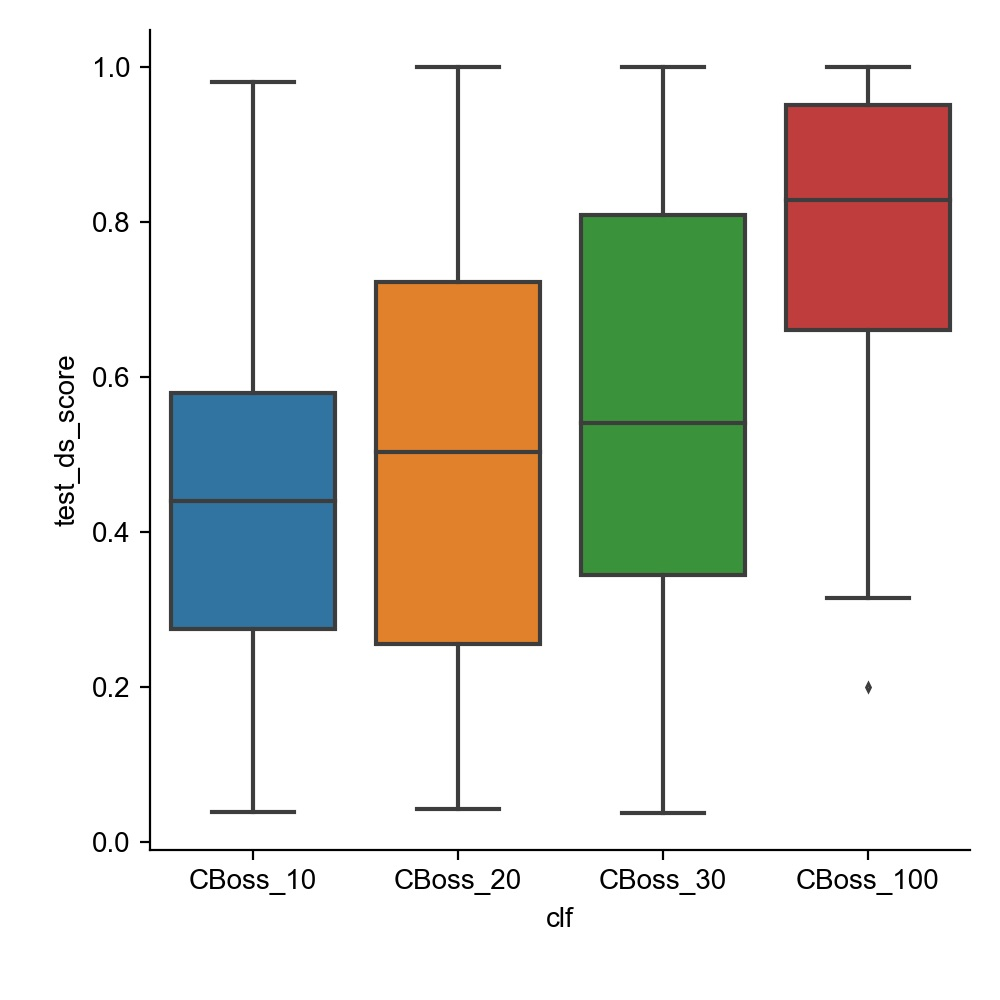
\includegraphics[width=0.49\textwidth,keepaspectratio]{boxplot_accuracy_CBoss.jpg}
  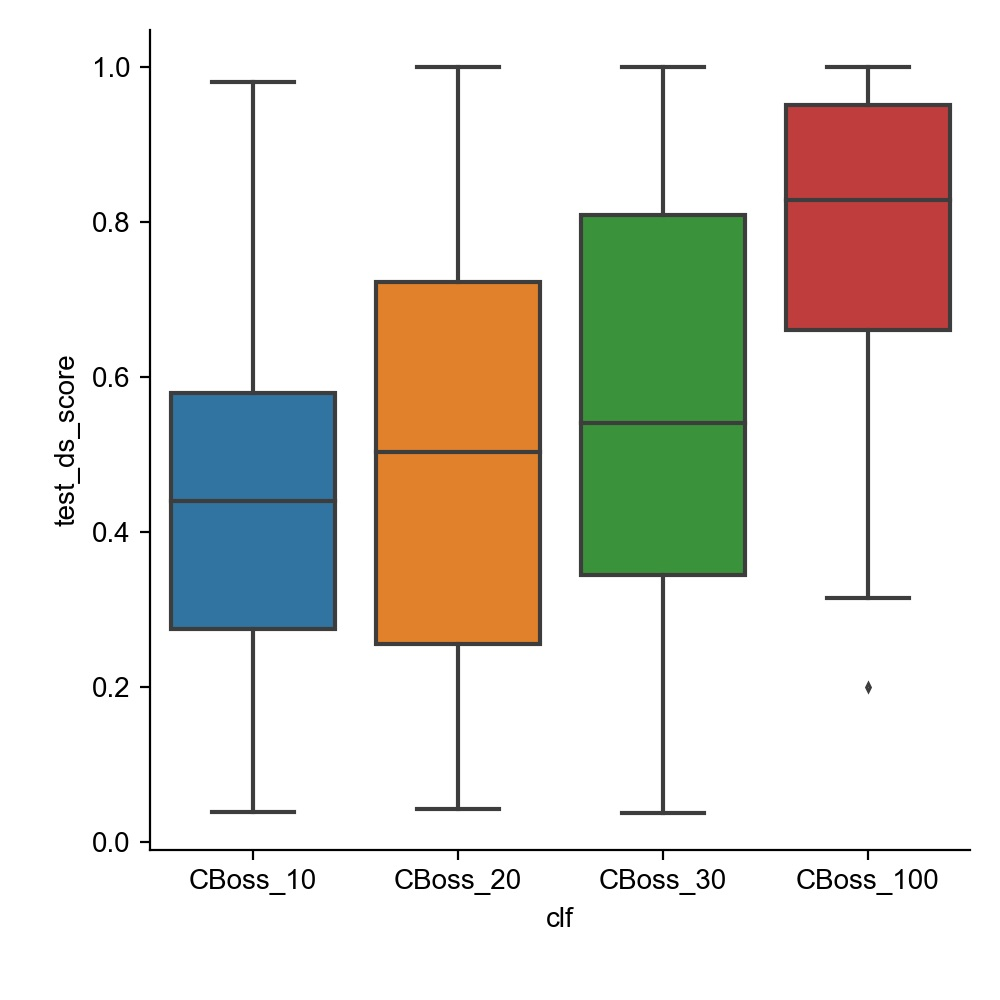
\includegraphics[width=0.49\textwidth,keepaspectratio]{boxplot_accuracy_CBoss.jpg}
  \caption{Metadata of the used data sets}
  \label{fig:FBeta1}
\end{figure}

By checking the boxplots for the $F_{1}$, we find that the median value for the 10\% version is \textbf{0.83}, while the median value of the 100\% version is \textbf{0.708}.
Also the distribution of the values for the 10\% version is very close to the median and the minimum value is higher than the median of the 100\% version.
Which means that even for the data sets on which the 10\% version of CBoss scores very low accuracy scores, it will still get a high $F_{1}$ relative to the 100\% version.
The harmonic mean over-compensates for the lower accuracy scores with very high values for earliness causing misleading values.

In order to decide which $\beta$ value is best to use, we carried out a sequence of experiments using $\beta$ = [0.1, 0.9].
The value that gave the most reasonable results was 0.5.
Figure shows the same comparison between the boxplots of $Balanced Accuracy$ and $F_{\beta}-measure$ for CBoss but with $\beta$ = 0.5.
Still $F_{1}$ allows for compensation between accuracy and earliness for the 10\% version, but it refines the values.
The median value for the 10\% version became \textbf{0.705} while that of the 100\% is \textbf{0.795}.
The distribution of values for the 10\% is spread more and the maximum value is falling near the median value of the 100\%.

\begin{figure}[!htbp]
  \captionsetup{justification=raggedright}
  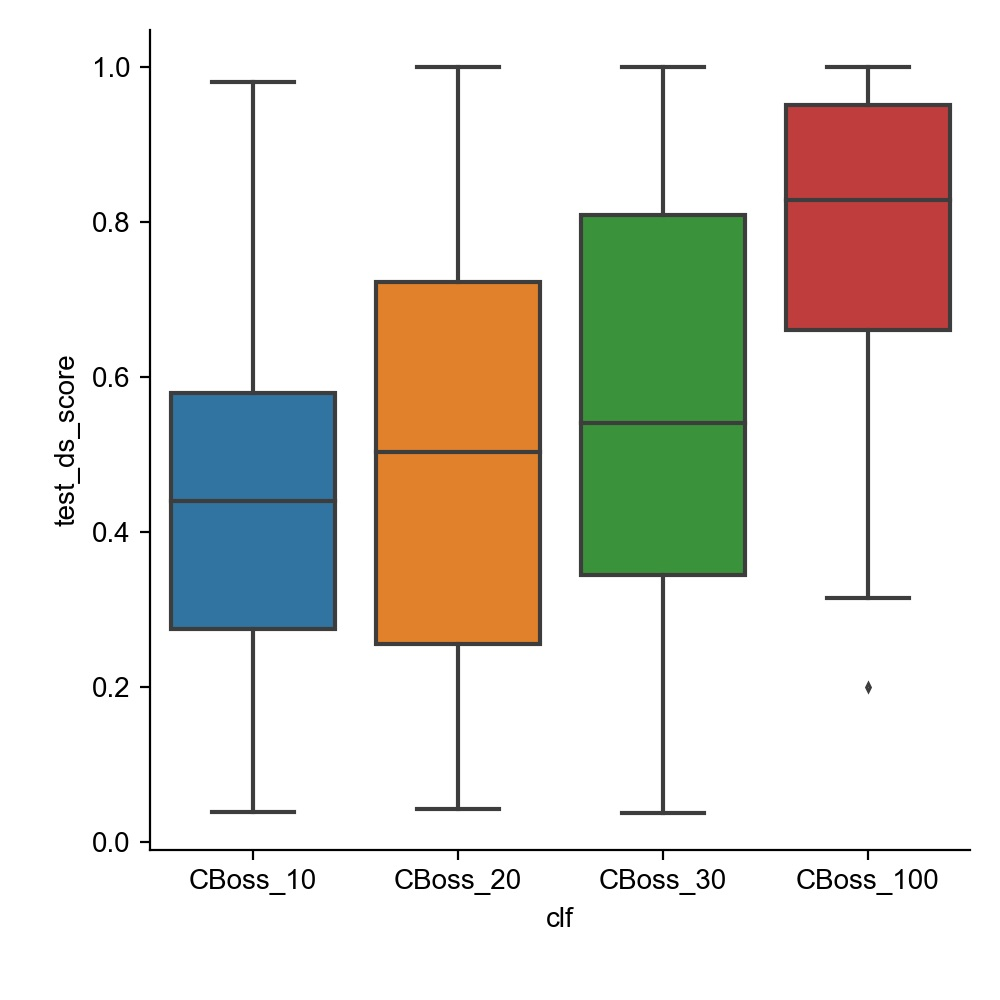
\includegraphics[width=0.49\textwidth,keepaspectratio]{boxplot_accuracy_CBoss.jpg}
  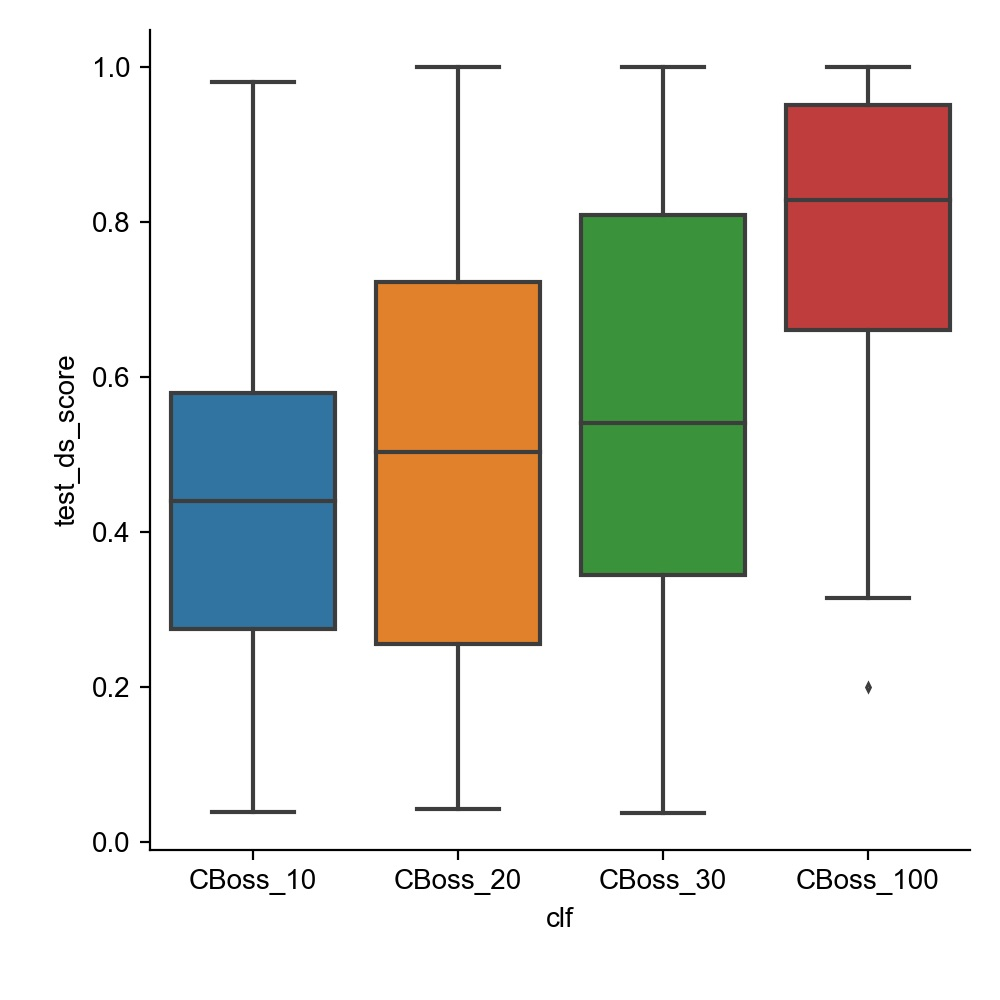
\includegraphics[width=0.49\textwidth,keepaspectratio]{boxplot_accuracy_CBoss.jpg}
  \caption{Metadata of the used data sets}
  \label{fig:FBeta1}
\end{figure}

We believe that selecting the best value of $\beta$ is not trivial.
It is problem dependant and not one specific value can fit for all problems.
For our experiments we decided to give earliness less priority than performance,
but in other situations it might be the case that both of them contribute with the same importance or even earliness is more critical.